\documentclass[usenames,dvipsnames,10pt,aspectratio=169]{beamer} 
% Add option 'aspectratio=169' for 16:9 widescreen 
% Add option  'handout' to ignore animations
% If you have a smaller amount of text, feel free to also try '11pt'! / Jesper

\usepackage[utf8]{inputenc}
\usepackage{verbatim}
\usepackage{minted}
\usepackage{graphicx}
\usepackage{wrapfig}
\usepackage{geometry}
\usepackage{listings}
\usepackage{color, xcolor}
\usepackage[document]{ragged2e}
\usetheme{umu}

\usemintedstyle{monokai}

\usepackage{hyperref}
\hypersetup{
    colorlinks=true,
    linkcolor=ucugreyish,
    filecolor=ucured,
    urlcolor=ucublue,
}
\urlstyle{same}

\lstdefinestyle{codestyle}{
    commentstyle=\color{ucugreyish},
    keywordstyle=\color{codeblue},
    numberstyle=\tiny\color{codegrey},
    stringstyle=\color{codepurple},
    basicstyle=\ttfamily\footnotesize,
    breakatwhitespace=false,         
    breaklines=true,                 
    captionpos=b,                    
    keepspaces=true,                 
    numbers=left,                    
    numbersep=5pt,                  
    showspaces=false,                
    showstringspaces=false,
    showtabs=false,                  
    tabsize=2
}

% %%% Bibliography
% \usepackage[style=authoryear,backend=biber]{biblatex}
% \addbibresource{bibliography.bib}

% \DeclareNameAlias{author}{given-family}

% %%% Suppress biblatex annoying warning
% \usepackage{silence}
% \WarningFilter{biblatex}{Patching footnotes failed}

%%% Some useful commands
% pdf-friendly newline in links
\newcommand{\pdfnewline}{\texorpdfstring{\newline}{ }} 
% Fill the vertical space in a slide (to put text at the bottom)
\newcommand{\framefill}{\vskip0pt plus 1filll}

%%% Enter additional packages below (or above, I can't stop you)! / Jesper
\renewcommand{\proofname}{\sffamily{Proof}}

% presentation template slides usage
% \framecard[color (not working)]{textbuf}
% \framesplit{Header}{picture}{textbuf}
% \framepic{image}{text}

% \begin{frame}[fragile]
% \lstset{style=codestyle}
% \begin{lstlisting}[language=Python, caption=Python example]
% import numpy as np
    
% def incmatrix(genl1,genl2):
%     m = len(genl1)
%     n = len(genl2)
%     M = None #to become the incidence matrix
%     VT = np.zeros((n*m,1), int)  #dummy variable
    
%     #compute the bitwise xor matrix
%     M1 = bitxormatrix(genl1)
%     M2 = np.triu(bitxormatrix(genl2),1) 

% \end{lstlisting}
% \end{frame}

%%%%%%%%%%%%%%%%%%%%%%%%%%%%%%%%%%%%%%%%%%%%%%%%%%%%%%%%%%%%%%%%%%%%%%%%%%%%%%%%%%%%%
\title{Linux course}
\subtitle{Shell}
\date[\today]{\small\today}
\author[Morhunenko Mykola]{Morhunenko Mykola}
\institute{APPS@UCU}

\begin{document}

\begin{frame}
\titlepage
\end{frame}

\begin{frame}{\contentsname}
\setbeamercolor{background canvas}{bg=ucugrey}
\tableofcontents
\end{frame}

\section{What Command Shell is?}
\framecard{What Command Shell is?}

\begin{frame}{What is command Shell?}
\begin{itemize}
    \item Command Shell is a computer program, that provide the user with a (CLI) command line interface to control the computer using keyboard, without GUI (Graphical user interface), for communication with the Linux system
    \item If you are using Linux, you have definitely see the command prompt. Usually it looks like {\color{ucugreen}\$} or, probably, {\color{ucugreen} \text{[username@hostname path] }\$}
    \item From the very beginning it looks like GUI is faster, but it is totally false: CLI just have high entry threshold. But it allows to write scripts (files with shell commands) that can automate routine, which is impossible in GUI
    \item Much more programs provide only CLI. If you want to use servers, connect to other computers via ssh, to be a real programmer, you must know shell
    \item You can check your shell by the command {\color{ucugreen} \$ echo \$SHELL}
    \item Most likely you have {\color{ucugreen} bash}, the most popular and stable one
    \item If you are done, you can leave the shell with {\color{ucugreen} exit} command, or by pressing the {\color{ucugreen}Ctrl+d} in the terminal emulator window
\end{itemize}
\end{frame}

\begin{frame}{What is Bash}
\begin{itemize}
    \item Bash stands for "Bourne(born)-again-shell"
    \item It is default shell for most Linux distros
    \item POSIX standard have a full description of the shell. Bash implements all this features, plus something own, known as {\color{ucugreen} bashism}
    \item Bash is a standard shell for the majority of  Linux distros, but it doesn't mean it is the best one
\end{itemize}
\end{frame}

\begin{frame}{ZSH}
    \begin{itemize}
        \item Zsh stands for {\color{ucugreen}Z-shell}
        \item Like Bash, it derives from Bourne family of shells, in everyday usage zsh is the same, as {\color{ucugreen} bash}, but have a lot of extensions and other syntax of configuration files (default - {\color{ucugreen}~/.zshrc})
        \item There is an entire eco-system of configuration tools and themes called oh-my-zsh which is very popular
        \item Also there are a huge amount of extensions at the github, that can make everyday usage easier - from auto-complete to syntax highlighting
        \item also there are differences in scripts, about it is later.
        
    \end{itemize}
\end{frame}


\section{Paths}
\framecard{Paths}
\begin{frame}{Path}
    \begin{itemize}
        \item  {\color{ucugreen} Path} - one of the most important terms in this topic (and in understanding, how programs work)
        \item Current path - or current directory, working directory - the directory, from where you are working, launching programs/scripts
        \item Paths can be absolute or relative
        \item Absolute
            \begin{itemize}
                \item {\color{ucugreen} /} - also known as  {\color{ucugreen} root path}, all paths that starts from it are {\color{ucugreen} absolute}. Other examples:
                \item {\color{ucugreen} /home/username}
                \item {\color{ucugreen} /usr/local/share/zsh/site-functions/}
            \end{itemize}
        \item Relative
            \begin{itemize}
                \item Relative paths don't starts from the root. Shell interpreter always run all programs with respect to the current path. They never begins with \ex{/}
                \item {\color{ucugreen} .zshrc}
                \item {\color{ucugreen} Documents/UCULinux/presentations}
            \end{itemize}
    \end{itemize}
\end{frame}
\begin{frame}{Path}
    \begin{itemize}
        \item Names are case-sensitive, that means {\color{ucugreen} /home/UserName} and {\color{ucugreen} /home/username} are different names
        \item There are also special paths
        \begin{itemize}
            \item {\color{ucugreen} ./} stands for the current path
            \item {\color{ucugreen} ../} stands for the path one step back. For example, if the {\color{ucugreen} ./} is {\color{ucugreen} /home/username}, the {\color{ucugreen} ../} will be {\color{ucugreen} /home}
            \item {\color{ucugreen} \textasciitilde /} stands for the directory of current user. For example, for {\color{ucugreen} root} user {\color{ucugreen} ~/} will be {\color{ucugreen} /root}, and for {\color{ucugreen} username} it will be {\color{ucugreen} /home/username}
        \end{itemize}
    \end{itemize}
\end{frame}

\section{Bash Intro}
\framecard{Bash Intro}

\begin{frame}{Syntax}
    All default commands (programs) have very similar syntax
    \begin{examples}
    \text{program\_name [option]... [arguments]...}
    \end{examples}
    Options starts from \ex{-} or \ex{-{}-} \newline
    To see, how to use any command
    \begin{examples}
        \text{program\_name -h} \newline or
        \text{program\_name -{}-}help \newline behind are synonyms, but parameter is in short and long form \newline
        man \text{program\_name}  - it provides full documentation about the command
    \end{examples}
\end{frame}

\begin{frame}{Base commands}
\begin{itemize}
    \item \ex{pwd} - print working directory - show your current path
    \item \ex{ls <path>} - list - show what is inside the directory
    \item \ex{cd [path]} - change directory - change your current directory
\end{itemize}
So now it is possible to get something 
\begin{examples}
    username\$ pwd \newline
    \ex[ucugrey]{> /home/username} \newline
    username\$ ls \newline
    \ex[ucugrey]{> Desktop Documents Downloads Music Pictures Videos} \newline
    username\$ cd Downloads \newline
    username\$ pwd \newline
    \ex[ucugrey]{> /home/username/Downloads}
\end{examples}
\end{frame}
\begin{frame}{Base commands}

{\Large{Introducing ls}} \newline
\begin{itemize}
    \item \ex{ls -a} - list all, including names starting with dot symbol "."
    \item \ex{ls -l} - list using a long list format, to display more information including permissions, size and important dates
    \item \ex{ls -r} - list in reversed order
    \item \ex{ls -R} - list current directory and all subdirectories recursively
    \item \ex{ls -S} - sort by file size, largest first
    Also they can be combined. The most commonly used
    \item \ex{ls -la} - list all with full info
    And the command have path as an argument, so the following command is also valid
    \item \ex{ls -la /etc/systemd/system}
\end{itemize}
And there are much more options, that can be found using \ex{ls -{}-help}
\end{frame}

\begin{frame}{Base commands}
    Now you can move around and see, what is around. But to work on your labs or projects, you need to create something and see, what is inside, and somehow manipulate it: \newline
    \begin{itemize}
        \item \ex{mkdir [dirname]} - make directory - create a new directory
        \item \ex{touch [filename]} - create a file with filename or update the date of file's last modification to current date
        \item \ex{date} - print current date and time
        \item \ex{echo [text]} - print the text to the standard output
        \item \ex{cat [filename]} - short for concatenate - show the file content
        \item \ex{cp [source...] [destination]} - copy - copy all from source (all arguments except the last) to the destination (the last argument). \ex{-r} option required for directories
        \item \ex{mv [source...] [destination]} - move - move all from source to destination
        \item \ex{rm [path]} - remove - remove the file. \ex{-rf} required for directories
    \end{itemize}
\end{frame}

\begin{frame}{Going deeper}

    {\Large Creating Links} \newline
    In Linux there are two types of links: hard and symbolic
    \begin{itemize}
        \item Inode - a data structure in the Unix-style file systems, that describes a file-system object
        \item Inode can have any number of hard links, and the inode will persists on the system until all hard links disappear. Changing in one file apply this changes also to all it's hard links
    \end{itemize}
\end{frame}

\begin{frame}{Going deeper}
    \begin{itemize}
        \item \ex{ls -i} command is used to list all files with it's inodes
        \item \ex{ln [source] [destination]} is used to create hard links
        \begin{examples}
            username \$ ln file1 file2 \newline
            username \$ ls -i \newline
            \ex[ucugrey]{> 9700529 file1  9700529 file2}
        \end{examples}
        as far as wee can see, both files have same inode
        \begin{examples}
        username \$ echo "Hello Wrold!" >> file1 \newline
        username \$ cat file2 \newline
        \ex[ucugrey]{> Hello World!}
        \end{examples}
        So changes in one file apply this changes to the other one \newline
    \end{itemize}
\end{frame}

\begin{frame}{Going deeper}
    What about symbolic links?
    \begin{itemize}
        \item symbolic links (symlinks) are used more often. This is a special type, and the link refers to another file by name, not by inode.
        \item deleting the source file will make the symlink broken
        \item \ex{ln -s} - used to create the symbolic link
        \begin{examples}
        username \$ ln -s file1 file3 \newline
        username \$ ls -l \newline
        
        > -rw-rw-r-- 2 username groupname 18 Apr 17 00:47 file1 \newline
        \, \, -rw-rw-r-- 2 username groupname 18 Apr 17 00:47 file2 \newline
        \, \, lrwxrwxrwx 1 username groupname  5 Apr 17 00:54 file3 -> file1
        \end{examples}
        \item Symlinks can be created to any type of file system objects
        \item Can be used to point to an object from another file system
    \end{itemize}
\end{frame}

\begin{frame}{Going deeper}

    {\Large Wildcards, Globs}
    \begin{itemize}
        \item In case, there is a folder with 25 test files, but it is necessary to delete first 8 of them... there are few ways, how to deal with that
        \begin{examples}
        username \$ rm test1 test2 test3 test4 test5 test6 test7 test8 \newline
        \,\,\,or... \newline
        username \$ rm test[1-8] \newline
        \,\,\,or if you want to delete all tests... \newline
        username \$ rm test*
        \end{examples}
        \item So, \ex{*} wildcard stands for all matches, any number of any symbol
        \item \ex{?} stands for \ex{any one symbol}
        \item \ex{[]} wildcard stands for ranges, so \ex{[abc]} means "any of a, b, c", the same for [a-c]
        \item \ex{!} stands for non-match, so [!a] stands for any symbol except 'a'
    \end{itemize}
\end{frame}

\begin{frame}{Going deeper}

    {\Large Important about wildcards}
    \begin{itemize}
        \item Be careful while using wildcards
        \item Bash preprocess all input to extend it with respect to wildcards
        \item so if you want to use one of such symbols just as symbols, you can either escape character with \ex{\textbackslash} symbol, or use single quotes
        \begin{examples}
        username \$ echo [fo]* > ./new\_file \newline in this case you will add names of all files starts with 'f' or 'o' \newline
        username \$ echo '[fo]*' > ./new\_file\newline
        username \$ echo \textbackslash [fo\textbackslash ]\textbackslash * > ./new\_file \newline
        both approaches above are correct
        \end{examples}
        \item \ex{ All bash commands are \href{https://ss64.com/bash/}{here}}
    \end{itemize}
\end{frame}

\section{Permissions}
\framecard{Permissions}

\framesplitc{Extensions}{graphics/ext.jpg}{
    \begin{itemize}
        \item The Linux world doesn't need file extensions
        \item The operating system doesn't use them to determine how to open a file
        \item But extensions are used by some parts of the OS to determine which program to use to open file
        \item So how the operating system find out, what the file is and how to deal with it?
    \end{itemize}
}

\begin{frame}{Permissions}
    \begin{itemize}
        \item When executing the \ex{ls -l} command, at the very beginning of every line there is 10 characters and then two words
        \begin{examples}
        username \$ ls -la \newline
        \ex[ucugrey]{> drwxrwxr-x 10 username groupname 4096 Apr 20 02:21 example\_directory} \newline
        \ex[ucugrey]{\,\,\, -rw-rw-r-{}- \hspace{0.2cm} 10 username groupname 4096 Apr 20 02:21 example\_textfile} \newline
        \ex[ucugrey]{\,\,\, -rwxr-xr-x \hspace{0.25cm} 10 username groupname 4096 Apr 20 02:21 example\_binary\_file} \newline
        \end{examples}
        \item They are not just letters, there is a lot of information behind these 10 characters (or, actually, 3 decimal numbers)
    \end{itemize}
\end{frame}

\begin{frame}{Permissions}
    \begin{figure}
        \centering
        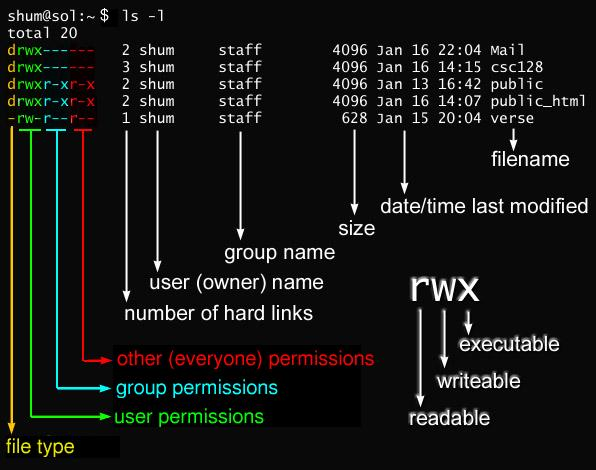
\includegraphics[height=0.8\paperheight]{graphics/permissions1.jpg}
\end{figure}
    
\end{frame}


\framesplitc{Permissions}{graphics/permissions.png}{
    \begin{itemize}
        \item The very first letter stands for file type, about them the info will be in the Filesystems topic
        \item To change permissions, there is a command \ex{chmod}
        \item To see all possible parameters, use \ex{chmod --help}. (But some explanations for the beginners are on the next page)
        \item All triplets of permissions \ex{rwx} have it's number correspondences
    \end{itemize}
}

\begin{frame}{Permissions}
    \begin{itemize}
        \item So in the help of \ex{chmod} are a little bit confusing things
        \item In \ex{[ugoa]} - User, Group, Other users, All
        \item In \ex{[rwxXst]} - Read, Write, eXecute
        \item eXecute only if the file is a directory or already has execute permission for some user
        \item Set user or group ID on execution
        \item Save program text on swap device (a performance enhancer)
    \end{itemize}
\end{frame}

\section{Scripts}
\framecard{Scripts}

\section{Sources}
\framecard{The end =)}
\framecard{Sources}
\begin{frame}{Sources}
\begin{itemize}
    \item \href{https://cms.ucu.edu.ua/pluginfile.php/181565/mod_resource/content/3/os_p01_bash.pdf}{Bash presentation for Operating systems course, UCU, Oleg Farenyuk (only from UCU domain)}
    \item \href{https://www.funtoo.org/Linux_Fundamentals,_Part_1}{Linux basics from the founder of Gentoo, Daniel Robbins, Chris Houser, Aron Griffis}
    \item \href {https://scriptingosx.com/}{Scripting OS X}
\end{itemize}    
\end{frame}

\end{document}